\section{Introduction}
\label{sec:introduction}

% state the learning objective 
The objective of this laboratory assignment is to study the circuit that can be seen if Figure~\ref{fig:T1Circuit}.
 
The circuit is composed by eleven components. This include two voltage sources (one of which is independent and the other current-controlled), two current sources (one independent and another voltage-controlled) and seven resistors. Furthermore, the circuit contains thirteen meshes (of which four of them are essential) and eight nodes.

In Section~\ref{sec:analysis}, a theoretical analysis of the circuit is
presented. In Section~\ref{sec:simulation}, the circuit is analysed by
simulation, and the results are compared to the theoretical results obtained in Section~\ref{sec:analysis}. The conclusions of this study are outlined in
Section~\ref{sec:conclusion}.

\vspace{4.0cm}

\begin{figure}[h] \centering
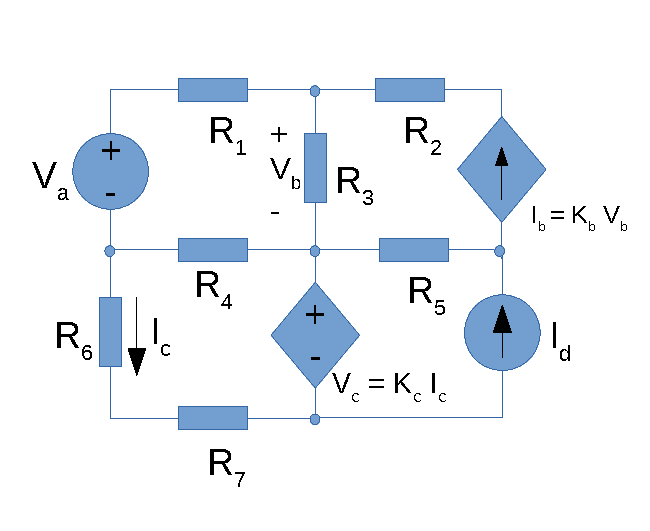
\includegraphics[width=0.8\linewidth]{T1Circuit.pdf}
\caption{Studied circuit.}
\label{fig:T1Circuit}
\end{figure}
